% BEGIN LICENSE BLOCK
% Version: CMPL 1.1
%
% The contents of this file are subject to the Cisco-style Mozilla Public
% License Version 1.1 (the "License"); you may not use this file except
% in compliance with the License.  You may obtain a copy of the License
% at www.eclipse-clp.org/license.
%
% Software distributed under the License is distributed on an "AS IS"
% basis, WITHOUT WARRANTY OF ANY KIND, either express or implied.  See
% the License for the specific language governing rights and limitations
% under the License.
%
% The Original Code is  The ECLiPSe Constraint Logic Programming System.
% The Initial Developer of the Original Code is  Cisco Systems, Inc.
% Portions created by the Initial Developer are
% Copyright (C) 2006 Cisco Systems, Inc.  All Rights Reserved.
%
% Contributor(s):
%
% END LICENSE BLOCK
%
% $Id: umsdebug.tex,v 1.10 2012/02/06 13:14:41 jschimpf Exp $
%

\chapter{Debugging}
%HEVEA\cutdef[1]{section}
\label{chapdebug}

\section{The Box Model}
\label{boxmodel}

The {\eclipse} debugger is based on a port model which is an extension
of the classical Box Model commonly used in Prolog debugging.

A procedure invocation (or goal) is represented by a box with entry
and exit ports.  Each time a procedure is invoked, a box is created
and given a unique invocation number.  The invocations of subgoals of
this procedure are seen as boxes inside this procedure box.

\begin{figure}
% The picture has been made with xfig and exported in
% encapsulated postscript mode
%\psfig{figure=boxmodel.ps}
\begin{center}
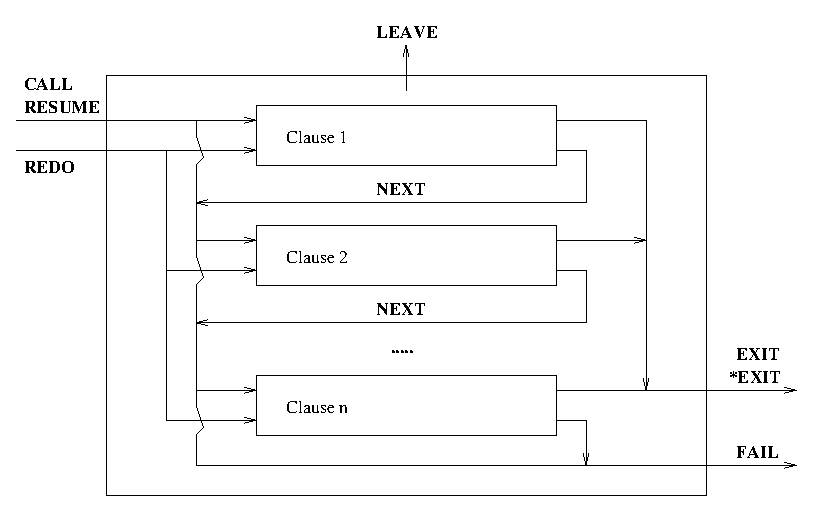
\includegraphics{boxmodel.eps}
\end{center}
\caption{The box model}
\end{figure}

Tracing the flow of the execution consists in tracing the crossing of
the execution flow through any of the port of the box.

The five basic ports of the box model of {\eclipse} are the CALL, EXIT,
REDO, FAIL and NEXT ports, the suspension facilities are traced through
the DELAY and RESUME ports, and the exceptional exit is indicated by LEAVE.

\begin{description}

\item[CALL:] When a procedure is invoked, the flow of the execution
enters the procedure box by its CALL port and enters the first clause
box which could (since not all clauses are tried, some of them being
sure to fail, i.e., indexing is shown) unify with the goal.
It may happen that a procedure is
called with arguments that make it sure to fail (because of
indexing). In such cases, the flow does not enter any clause box.

For each CALL port a new procedure box is created and is given:
\begin{itemize}
\item an \emph{invocation number} that is one higher than that given for
the most recent CALL port. This allows to uniquely identify a
procedure invocation and all its corresponding ports.

\item a \emph{level} that is one higher than that of its parent goal.
\end{itemize}

The displayed variable instantiations are the ones at call time,
i.e., before the head unification of any clause.

\item[EXIT:] When a clause of a predicate succeeds (i.e., unification
succeeded and all procedures called by the clause succeeded),
the flow gets out of the box by the EXIT port of both boxes (only
the EXIT port of the \emph{procedure box} is traced).

When a procedure exits non-deterministically (and there are still
other clauses to try on that procedure or one of its children goals
has alternatives which could be resatisfied), the EXIT port is traced
with an asterisk (*EXIT). When the last possibly matching clause of a
procedure is exited, the exit is traced without asterisk. This means
that this procedure box will never be retried as there is no other
untried alternative.

The instantiations shown in the EXIT port are the ones at exit time,
they result from the (successful) execution of the procedure.

\item[FAIL:] When a clause of a procedure fails (because head unification
failed or because a sub-goal failed), the flow of the execution exits
the clause box and leaves the procedure box via the FAIL port.
Note that the debugger cannot display any argument information at
FAIL ports (an ellipsis \verb:...: is displayed instead for each argument).

\item[NEXT:] If a clause fails and there is another possibly
matching clause to try, then that one is tried for unification.
The flow of the execution from the failure of one clause to the
head unification of a following clause is traced as a NEXT port.
The displayed variable instantiations are the same as those of the
corresponding CALL or REDO port.

\item[ELSE:]
This is similar to the NEXT port, but indicates that the next branch of a
\biptxtref{disjunction (;/2)}{;/2}{../bips/kernel/control/O-2.html}
it tried after the previous branch failed.
The predicate that gets displayed with the port is the predicate
which contains the disjunction (the immediate ancestor).

\item[REDO:] When a procedure box is exited trough an *EXIT port,
the box can be retried later to get a new solution. This will happen when a
later goal fails. The backtracking will cause failing of all
procedures that do not have any alternative, then the execution flow
will enter a
procedure box that an contains alternative through a REDO port.

Two situations may occur: either the last tried clause has called a
procedure that has left a choice point (it has exited through an
*EXIT port). In that case the nested procedure box is re-entered
though another REDO-port.

Otherwise, if the last clause tried does not contain any
nondeterministically exited boxes, but there are other untried clauses
in the procedure box, the next possibly matching clause will be tried.

The last REDO port in such a sequence is the one which contains the
actual alternative that is tried. The variable instantiations for all
REDO ports in such a sequence are the ones corresponding to the call
time of the last one.

%\item[UNIFY:] When a clause head successfully unifies with
%a called goal, a UNIFY port is traced to show the result of the
%unification. However, this port is not traced for unit clause since it
%is identical to the EXIT port.
%
%Please note that this port is not shown in the default settings but it
%can be switched on with the appropriate
%\bipref{set_leash/2}{../bips/kernel/debug/set_leash-2.html} call.

\item[LEAVE:]
This port allows to trace the execution of exceptions.  Exceptions
are either raised implicitly by built-in predicates (in which case the
built-in itself exits via the LEAVE port), or explicitly through a call to
\bipref{throw/1}{../bips/kernel/control/throw-1.html}
(or \bipref{exit_block/1}{../bips/kernel/control/exit_block-1.html}).
All ancestors of the predicate that raised the exception will subsequently
exit via a LEAVE port, until a
\bipref{catch/3}{../bips/kernel/control/catch-3.html}
(or \bipref{block/3}{../bips/kernel/control/block-3.html})
is found, whose second argument matches the exception.
This invocation of
\bipref{catch/3}{../bips/kernel/control/catch-3.html}
then passes a NEXT port (at which point the exception has been caught),
and then execution continues via a normal call of the recovery goal
(the third argument of the
\bipref{catch/3}{../bips/kernel/control/catch-3.html}).

As with the FAIL port, no argument values are displayed in the LEAVE port.

%\item[CUT:] The cut is considered by the debugger as a predicate
%(it has its own box with a CALL and an EXIT port) that always
%succeeds.  The side effects it causes are traced through the CUT port.
%Each goal whose choice point is removed are traced with a CUT port.
%This port is actually not a real procedure port, it only notifies of
%the destruction (performed by the cut) of the choice point of a goal.
%When a goal has been cut, it can not be re-satisfied.  Therefore, the
%flow of the execution will never re-enter the procedure box through
%its REDO port. The displayed variable instantiations are the current
%ones.
%
%By default, the debugger only prints this port, but does not prompt for
%a command. This can be changed using
%\bipref{set_leash/2}{../bips/kernel/debug/set_leash-2.html}.
%
%\item[TRY:] The procedure creates a choicepoint. By default, the debugger does
%not show this port. Use
%\bipref{set_leash/2}{../bips/kernel/debug/set_leash-2.html} to make it
%visible.

\item[DELAY:]
The displayed goal becomes suspended. This is a singleton port, it does
not enter or leave a box. However, a new \emph{invocation number} is assigned
to the delayed goal, and this number will be used in the matching RESUME port.
The DELAY port is caused by one of the built-in predicates
\bipref{suspend/3}{../bips/kernel/suspensions/suspend-3.html},
\bipref{suspend/4}{../bips/kernel/suspensions/suspend-4.html},
\bipref{make_suspension/3}{../bips/kernel/suspensions/make_suspension-3.html}
or a delay clause.
The port is displayed just after the delayed goal has been created.

\item[RESUME:] When a waking condition causes the resuming of
a delayed goal, the procedure box is entered through its RESUME
port.  The box then behaves as if it had been entered through its CALL
port.  The invocation number is the same as in its previous DELAY port.
which makes it easy to identify corresponding delay and resume events.
However the depth level of the RESUME corresponds to the waking situation.
It is traced like a subgoal of the goal which has caused the waking.

\end{description}

In the rest of this chapter the user interface to the debugger is
described, including the commands available in the debugger itself as
well as built-in predicates which influence it.  Some of the debugger
commands are explained using an excerpt of a debugger session.  In
these examples, the user input is always underlined (it is in fact
not always output as typed) to distinguish it from the computer output.

\subsection{Breakpoints}

Breakpoints can be set on specific calls to a predicate, i.e., on a specific
body goal in the source, so that the
debugger will stop only at a CALL port only when that specific body goal is
executed. A breakpoint is specify by giving the source file and the line
number where the body goal is.

For example, if the following predicate is in a file called \notation{newtop},
with the following line numbers:

\begin{verbatim}
  243  check_words([],[]).
  244  check_words([Word|Words],[RevWord|RevWords]) :-
  245     check_words(Words,RevWords).
\end{verbatim}

The breakpoint for the body goal \notation{check_words(Words, RevWords)} would
be \notation{newtop:245}. Note that the file name must be sufficiently specified
for ECLiPSe to find the file from your current working directory.

For a call that has a breakpoint set, the execution will stop when the call
is made, i.e., at the CALL port for that specific body goal.

\section{Format of the Tracing Messages}
All trace messages are output to the
\notationidx{debug_output} stream.

The format of one trace line is as follows:
\begin{quote}
\begin{verbatim}
S+(4) 2 *EXIT<5> module:foo(one, X, two)   %>
12 3  4 5 6   7    8       9              10
\end{verbatim}
\end{quote}

\begin{enumerate}
\item The first character shows some properties of the
displayed procedure.
It may be one of
\begin{itemize}
\item C - an external procedure, not implemented in Prolog
\item S - a \emph{skipped} procedure, i.e., a procedure whose
subgoals are not traced
%\item N - a procedure compiled in non-debug mode, i.e., behaves like skipped.
\end{itemize}

\item A \notation{+} displayed here shows that the procedure has a spy point
  set,
  and a \notation{\#} shows that the specific call has a break-point set.
\index{spy point}

\item The number between parentheses shows the box invocation number
of this procedure call.  Since each box has a unique invocation
number, it can be used to identify ports that belong to the same box.
It also shows how many procedure redos have been made since the
beginning of the query.  Only boxes that can be traced obtain an
invocation number, for instance subgoals of a procedure which is
compiled in debug mode or has its skip-flag set are not numbered.

When a delayed goal is resumed, it keeps the invocation number it was
assigned when it delayed.  This makes it easy to follow all ports of a
specified call even in data-driven computation.

\item The second number shows the level or depth of the goal,
i.e., the number of its ancestor boxes.  When a subgoal is called, the
level increases and after exit it decreases again.  The initial level
is 1.

Since a resumed goal is considered to be a descendant of the procedure
that woke it, the level of a resumed goal may be different from
the level the goal had when it delayed.

\item An asterisk before an \notation{EXIT} means that this
procedure is nondeterministic and that it might be resatisfied.

\item The next word is the name of the port.
It might be missing if the displayed goal is not the current position
in the execution (e.g., when examining ancestors or delayed goals).

\begin{description}
\item[\notation{CALL}:] a procedure is called for the first time concerning a
  particular
invocation;

\item[\notation{DELAY}:] a procedure delays;

\item[\notation{EXIT}:] a procedure succeeds;

\item[\notation{FAIL}:] a procedure fails, there is no (other) solution;

\item[\notation{LEAVE}:] a procedure is left before having failed or exited
  because an exception was raised by either a built-in predicate error
condition or a call to \bipref{throw/1}{../bips/kernel/control/throw-1.html}
or \bipref{exit_block/1}{../bips/kernel/control/exit_block-1.html};

\item[\notation{NEXT}:] the next possibly matching clause of a procedure is
  tried
because unification failed or a sub-goal failed;

\item[\notation{ELSE}:] the next branch of a disjunction is tried because some
  goal
in the previous branch failed;

\item[\notation{REDO}:] a procedure that already gave a solution is called again
  for
an alternative;

\item[\notation{RESUME}:] a procedure is woken (the flow enters the procedure
  box as for
a call) because of a unification of a suspending variable.

%\item[UNIFY] unification succeeded (not shown for unit clauses).

\end{description}

\item This only appears if the goal is executing at a different priority
  than 12, the normal priority. The number between the angled brackets
  shows the priority (between 1 and 11) that the  goal is executed at.

\item For the tty debugger, the optional module name followed by a colon.
Printing of the module can be enabled and disabled by the debugger
command \notation{m}.\dbgcmdidx{m}{module}
If it is enabled, the module from where the procedure is called is
displayed.  By default the module printing is disabled. With tkeclipse, the
module name is not displayed with the traceline, instead, you can get the
information by right holding the mouse button over the trace line in the
call stack window.

\item The goal is printed according to the current instantiations
of its variables.  Arguments of the form \notation{...} represent subterms
that are not printed due to the depth limit in effect.
The depth limit can be changed using the
\notation{<}\dbgcmdidxPlus{$<$}{<}{print depth} command.

The goal is printed with the current \notation{output_mode} settings.
which can be changed using the
\notation{o}\dbgcmdidx{o}{output mode} command.

\item The prompt of the debugger, which means that it is waiting
for a command from the user. Note there is no prompt when tkeclipse tracer
is used.
\end{enumerate}

\section{Debugging-related Predicate Properties}

Predicates have a number of properties which can be listed using the
\bipref{pred/1}{../bips/kernel/env/pred-1.html} built-in.
The following predicate flags and properties affect the way the
predicate is traced by the debugger:
\begin{quote}
\begin{description}
\item[debugged]\mbox{}\\
        Indicates whether the predicate has been compiled in debug-compile mode.
        If \notation{on}, calls to the predicate's subgoal will be traced.
        The value of this property can only be changed by re-compiling
        the predicate in a different mode.

\item[leash]\mbox{}\\
        If \notation{notrace}, no port of the predicate will be shown
        in the trace (but the invocations will be counted nevertheless).
        If \notation{stop}, the ports of this predicate will be shown and
        the debugger will stop and await new commands.
        (The \notation{print} setting is currently not supported).
        The value of this property can be changed with
        \bipref{traceable/1}{../bips/kernel/debug/traceable-1.html},
        \bipref{untraceable/1}{../bips/kernel/debug/untraceable-1.html} or
        \bipref{set_flag/3}{../bips/kernel/compiler/set_flag-3.html}.

\item[spy]\mbox{}\\
        If \notation{on}, the predicate has a spy-point and the debugger will
        stop at its ports when in leap mode.
        The value of this property can be changed with
        \bipref{spy/1}{../bips/kernel/debug/spy-1.html},
        \bipref{nospy/1}{../bips/kernel/debug/nospy-1.html} or
        \bipref{set_flag/3}{../bips/kernel/compiler/set_flag-3.html}.

\item[skipped]\mbox{}\\
        If \notation{on}, the predicate's subgoal will not be traced even
        if it has been compiled in debug-compile mode.
        The value of this property can be changed with
        \bipref{skipped/1}{../bips/kernel/debug/skipped-1.html},
        \bipref{unskipped/1}{../bips/kernel/debug/unskipped-1.html} or
        \bipref{set_flag/3}{../bips/kernel/compiler/set_flag-3.html}.

\item[start_tracing]\mbox{}\\
        If \notation{on}, a call to the predicate will activate the debugger if
        it
        is not already running.
        Only the execution within this predicate's box will be traced.
        This is useful for debugging part of a big
        program without having to change the source code.
        The effect is similar to wrapping all call of the predicate into
        \bipref{trace/1}{../bips/kernel/debug/trace-1.html}.
\end{description}
\end{quote}


%{\it Leashing} stands for the way the trace lines of a
%procedure at a port are displayed and handled by the debugger.
%There are three distinct leash levels:
%
%\begin{description}
%\item[stop] Full leashing, the trace line is displayed, the debugger prints
%a prompt and waits for a command from the user.
%
%\item[print] The trace line is only displayed and the debugger
%does not stop but it continues to the next trace line.
%
%\item[notrace] The trace line is not displayed and
%the debugger does not prompt for a command.
%\end{description}
%The leashing mode can be specified separately for ports and procedures.
%The debugger command {\bf p} and
%\index{p --- port leashing (debugger cmd)}
%the predicate \bipref{set_leash/2}{../bips/kernel/debug/set_leash-2.html}
%are for ports, e.g.,
%\begin{quote}\begin{verbatim}
%set_leash(next, notrace).
%\end{verbatim}\end{quote}
%will suppress printing of all NEXT ports.
%To change the leash mode for a certain procedure,
%the predicate \bipref{set_flag/3}{../bips/kernel/compiler/set_flag-3.html} or
%the debugger command {\bf t}
%\index{t --- procedure trace mode (debugger cmd)}
%are used. For instance
%\begin{quote}\begin{verbatim}
%set_flag(p/3, leash, print).
%\end{verbatim}\end{quote}
%will cause all ports of the procedure p/3 to be printed, but the
%debugger will not stop or prompt for commands.
%For each trace line, the
%effective leash mode is combined from the mode of the current
%procedure and the current port and if the two are not equal, the more
%restrictive one is taken.
%
%A particularly useful combination is to set a spy point on a procedure
%\index{spy point}
%and set its leash mode to {\tt print}. This will cause the
%debugger to print a continuous trace of all ports involving this procedure.


\section{Starting the Debugger}

Several methods can be used to switch the debugger on.
If the textual interactive top-level is used, the commands
\bipref{trace/0}{../bips/kernel/debug/trace-0.html} and
\bipref{debug/0}{../bips/kernel/debug/debug-0.html} are used to
switch the debugger on for the following queries typed from the
top-level.
\bipref{trace/0}{../bips/kernel/debug/trace-0.html} will switch the
debugger to \notation{creep} mode whereas
\bipref{debug/0}{../bips/kernel/debug/debug-0.html} will switch it
in leap mode.

For the \tkeclipse{} graphical toplevel, the debugger may be switched on by
starting the tracer from the Tools menu before executing the query. This
puts the debugger in \notation{creep} mode.

When the debugger is in \notation{creep} mode, it will
prompt for a command at the crossing of the first
%leashed
port of a
leashed procedure.  When the debugger is in leap mode,
it will prompt for a command at the first port of a leashed
procedure that has a spy point.  The debugger is switched off either
from the toplevel with the commands
\bipref{nodebug/0}{../bips/kernel/debug/nodebug-0.html} or
\bipref{notrace/0}{../bips/kernel/debug/notrace-0.html}, or by
typing \notation{n} or \notation{N} to the debugger prompt.

A spy point can be set on a procedure, or a breakpoint on a specific call,
using
\bipref{spy/1}{../bips/kernel/debug/spy-1.html} (which will
\index{spy point} also switch the debugger to leap)
and removed
with \bipref{nospy/1}{../bips/kernel/debug/nospy-1.html}.  They
both accept a \about{SpecList} as argument.  Note that
\bipref{set_flag/3}{../bips/kernel/compiler/set_flag-3.html} can
be used to set and reset spy points without switching the debugger on
and without printing messages.

\bipref{debugging/0}{../bips/kernel/debug/debugging-0.html} can be
used to list the spied predicates and the current debugger mode.

\begin{quote}
\begin{verbatim}
[eclipse 1]: spy writeln/1.
spypoint added to writeln / 1.

yes.
Debugger switched on - leap mode
[eclipse 2]: debugging.
Debug mode is leap
writeln / 1 is being spied

yes.
[eclipse 3]: true, writeln(hello), true.
B+(2) 0  CALL   writeln(hello) %> l leap
hello
B+(2) 0  EXIT   writeln(hello) %> c creep
B (3) 0  CALL   true %> l leap

yes.
[eclipse 4]: trace.
Debugger switched to creep mode

yes.
[eclipse 5]: true, writeln(hello), true.
B (1) 0  CALL   true %> c creep
B (1) 0  EXIT   true %> c creep
B+(2) 0  CALL   writeln(hello) %> l leap
hello
B+(2) 0  EXIT   writeln(hello) %> l leap

yes.
\end{verbatim}
\end{quote}

\section{Debugging Parts of Programs}

\subsection{Mixing debuggable and non-debuggable code}

The debugger can trace only procedures which have been compiled in
debug mode.  The compiler debug mode is by default switched on and it
can be changed globally by setting the flag \notation{debug_compile} with the
\bipref{set_flag/2}{../bips/kernel/env/set_flag-2.html}
predicate or using
\bipref{dbgcomp/0}{../bips/kernel/obsolete/dbgcomp-0.html} or
\bipref{nodbgcomp/0}{../bips/kernel/obsolete/nodbgcomp-0.html}.
The global compiler debug mode can be overruled on a file-by-file basis
using one of the compiler pragmas
\begin{quote}
\begin{verbatim}
:- pragma(nodebug).
:- pragma(debug).
\end{verbatim}
\end{quote}
Once a program (or a part of it) has been
debugged, it can be compiled in \notation{nodbgcomp} mode so that all
optimisations are done by the compiler.  The advantages of
non-debugged procedures are

\begin{itemize}
\item They run slightly faster than the debugged procedures
when the debugger is switched off.  When the debugger is switched on,
the non-debugged procedures run considerably faster than the debugged
ones and so the user can selectively influence the speed of the code
which is being traced as well as its space consumption.

\item Their code is shorter than that of the debugged procedures.
\end{itemize}

Although only procedures compiled in the \notation{dbgcomp} mode can be
traced, it is possible to mix the execution of procedures in both
modes.  Then, calls of \notation{nodbgcomp} procedures from \notation{dbgcomp}
ones are
traced, however further execution within \notation{nodbgcomp} procedures,
i.e., the execution of their subgoals, no matter in which mode, is not
traced.  In particular, when a \notation{nodbgcomp} procedure calls a
\notation{dbgcomp}
one, the latter is normally not traced.
There are two important exceptions from this rule:
\begin{itemize}
\indextt{waking/1}
\item When a debuggable procedure has delayed and its DELAY port has
been traced, then its RESUME port is also traced, even when it is woken
inside non-debuggable code.
\index{\atsym/2@\notation{"@/2}}
\indextt{subcall/2}
\item When non-debuggable code \emph{meta-calls} a debuggable procedure
(i.e., via \bipref{call/1}{../bips/kernel/control/call-1.html}),
then this procedure can be traced.  This is a useful feature for the
implementation of meta- predicates like
\bipref{setof/3}{../bips/kernel/allsols/setof-3.html}, because it
allows to hide the details of the setof-implementation, while allowing
to trace the argument goal.
\end{itemize}

Setting a procedure to skipped (with
\bipref{set_flag/3}{../bips/kernel/compiler/set_flag-3.html} or
\bipref{skipped/1}{../bips/kernel/debug/skipped-1.html}
)
%or using the fast skip command of the debugger (\notation{F}) are also ways
is another way
to speed up the execution of procedures that need not be
debugged.  The debugger will ignore everything that is called inside
the skipped procedure like for a procedure compiled in \notation{nodbgcomp}
mode.  However, the debugger will keep track of the execution of a
procedure skipped with the command \notation{s} of the debugger so that it
will be possible to ``creep'' in it on later backtracking or switch the
debugger to \notation{creep} mode while the skip is running (e.g.,  by
interrupting a looping predicate with \notation{\^{}C} and switching to
\notation{creep} mode).

The two predicates
\bipref{trace/1}{../bips/kernel/debug/trace-1.html} and
\bipref{debug/1}{../bips/kernel/debug/debug-1.html} can be used to
switch on the debugger in the middle of a program.  They execute their
argument in \notation{creep} or \notation{leap} mode respectively.  This is
particularly useful when debugging large programs that take too much
time (or need a lot of memory) to run completely with the debugger.
\begin{quote}
\begin{verbatim}
[eclipse 1]: debugging.
Debugger is switched off

yes.
[eclipse 2]: big_goal1, trace(buggy_goal), big_goal2.
Start debugging - creep mode
  (1) 0  CALL   buggy_goal %> c creep
  (1) 0  EXIT   buggy_goal %> c creep
Stop debugging.

yes.
\end{verbatim}
\end{quote}

It is also possible to enable the debugger in the middle of execution
without changing the code.  To do so, use
\bipref{set_flag/3}{../bips/kernel/compiler/set_flag-3.html}
to set the \notationidx{start_tracing} flag of the predicate of interest.
Tracing will then start (in leap mode) at every call of this
predicate.\footnote{%
  Provided the call has been compiled in debug_compile mode,
  or the call is a meta-call.}
To see the starting predicate itself,
set a spy point in addition to the \notation{start_tracing} flag:
\begin{quote}
\begin{verbatim}
[eclipse 1]: debugging.
Debugger is switched off

yes.
[eclipse 2]: set_flag(buggy_goal/0, start_tracing, on),
             set_flag(buggy_goal/0, spy, on).

yes.
[eclipse 3]: big_goal1, buggy_goal, big_goal2.
 +(0) 0 CALL  buggy_goal   %> creep
 +(0) 0 EXIT  buggy_goal   %> creep

yes.
\end{verbatim}
\end{quote}

In tkeclipse, the debugger can also be started in this way. The tracer tool
will popup at the appropriate predicate if it has not been invoked
already. The \notation{start_tracing} flag can also be set with the predicate
browser tool.

%----------------------------------------------------------------------
\section{Using the Debugger via the Command Line Interface}
%----------------------------------------------------------------------
This section describe the commands available at the debugger prompt
in the debugger's command line interface (for the graphical user
interface, please refer to the online documentation).

Commands are entered by typing the corresponding key
(without newline), the case of the letters is significant.  The action
of some of them is immediate, others require additional parameters to
be typed afterwards.  Since the {\eclipse} debugger has the possibility to
display not only the goal that is currently being executed (the {\it
current} goal or procedure), but also its ancestors, some of the
commands may work on the \emph{displayed} procedure whatever it is, and
others on the \emph{current} one.
% Any undefined debugger command will reset the displayed procedure to the
% current one.

\subsection{Counters and Command Arguments}
Some debugger commands accept a counter (a small integer number)
before the command letter (e.g., \notation{c}, i.e., \notation{creep}).
The number is just prefixed to the command and terminated by the
command letter itself. If a counter is given for a command that
doesn't accept a counter, it is ignored.

When a counter is used and is valid for the command,
the command is repeated, decrementing the counter until zero.
When repeating the command, the command and the remaining counter
value is printed after the debugger prompt instead of waiting for user input.

Some commands prompt for a parameter, e.g., the \notation{j} (\notation{jump)}
command asks for the number of the level to which to jump.
Usually the parameter has a sensible default value (which is printed
in square backets). If just a newline is typed, then the default value
is taken. If a valid parameter value is typed, followed by newline,
this value is taken. If an illegal letter is typed, the command is aborted.


%----------------------------------------------------------------------
\subsection{Commands to Continue Execution}
%----------------------------------------------------------------------
All commands in this section continue program execution.
They difference between them is the condition under which execution
will stop the next time.  When execution stops again, the next trace
line is printed and a new command is accepted.

\begin{descr}{1cm}

\ncmd{c}{creep}\\
This command allows exhaustive tracing: the execution stops at the
next port of any leashed procedure.  No further parameters are
required, a counter \about{n} will repeat the command \about{n} times.
It always applies on the current procedure, even when the displayed
procedure is not the current one (e.g., during term inspection).
An alias for the \notation{c} command is to just type newline (Return-key).

\ncmd{s}{skip}\\
If given at an entry port of a box (CALL, RESUME, REDO), this command skips
the execution until an exit port of this box (EXIT, FAIL, LEAVE).
If given in an exit port it works like \notation{creep}.
(Note that sometimes the \notation{i} command is more appropriate, since it
skips to the next port of the current box, no matter which).
A counter, if specified, repeats this command.

%\ncmd{F}{fast skip}\\
%Is similar to the skip command \notation{s}. The difference is that the
%debugger does not keep track of the execution during the skip so that
%it is faster. As a result, it is not possible to {\it creep} later on
%inside this procedure (e.g., it will not be possible to 'creep'
%through this procedure on later backtracking, and switching the debugger
%back to {\it creep} mode using \^\space C while the skipped procedure is
%looping will have no effect).

\ncmd{l}{leap}\\
Continues to the next spy point (any port of a procedure
which has its spy flag set).
\index{spy point}
A counter, if specified, repeats this command.

\mcmd{i}{invocation skip}\\
Continue to the next port of the box with the invocation number
specified. The default invocation number is the one of the current box.
Common uses for this command are to skip from CALL to NEXT, from NEXT
to NEXT/EXIT/FAIL, from *EXIT to REDO, or from DELAY to RESUME.

\mcmd{j}{jump to level}\\
Continue to the next port with the specified nesting level (which can
be higher or lower than the current one).
The default is the parent's level, i.e., to continue until the current
box is exited, ignoring all the remaining subgoals of the current clause.
This is particularly useful when a \notation{c} (\notation{creep}) has been
typed where a \notation{s} (\notation{skip}) was wanted.

\cmd{n}{nodebug}\\
This command switches tracing off for the remainder of the execution.
However, the next top-level query will be traced again.
Use \notation{N} to switch tracing off permanently.

\cmd{q}{query the failure culprit}\\
The purpose of this command is to find out why a goal has failed (FAIL)
or was aborted with an exception (LEAVE).  It prints the invocation
number of the goal which caused the failure.  You can then re-run the
program in \notation{creep} mode and type \notation{q} at the first command
  prompt.  This will
then offer you to jump to the CALL port of the culprit goal.
%cannot quote: too wide
\begin{verbatim}
[eclipse 3]: p.
  (1) 1 CALL  p   %> skip
  (1) 1 FAIL  p   %> query culprit
failure culprit was (3) - rerun and type q to jump there   %> nodebug? [y]
No (0.00s cpu)

[eclipse 4]: p.
  (1) 1 CALL  p   %> query culprit
failure culprit was (3) - jump to invoc: [3]?
  (3) 3 CALL  r(1)   %> creep
  (3) 3 FAIL  r(...)   %> creep
  (2) 2 FAIL  q   %> creep
  (1) 1 FAIL  p   %> creep
No (0.01s cpu)
\end{verbatim}

\cmd{v}{var/term modification skip}\\
This command sets up a monitor on the currently displayed term,
which will cause a MODIFY-port to be raised on each modification to
any variable in the term. These ports will all have a unique invocation
number which is assigned and printed at the time the command is issued.
This number can then be used with the \notation{i} command to skip to where
the modifications happen.
%cannot quote: too wide
\begin{verbatim}
[eclipse 4]: [X, Y] :: 1..9, X #>= Y, Y#>1.
  (1) 1 CALL  [X, Y] :: 1..9   %> var/term spy? [y]
Var/term spy set up with invocation number (2)   %> jump to invoc: [1]? 2
  (2) 3 MODIFY  [X{[1..9]}, Y{[2..9]}] :: 1..9   %> jump to invoc: [2]?
  (2) 4 MODIFY  [X{[2..9]}, Y{[2..9]}] :: 1..9   %> jump to invoc: [2]?
\end{verbatim}
Note that these monitors can also be set
up from within the program code using one of the built-ins
\bipref{spy_var/1}{../bips/kernel/debug/spy_var-1.html} or
\bipref{spy_term/2}{../bips/kernel/debug/spy_term-2.html}.

%\cmd{v}{variable skip}\\
%This command allows to resume tracing when a specified variable
%becomes instantiated.  The debugger prompts for the name of the
%variable whose instantiation is looked for.  The variable identification is
%either its name or, in case it is not unique, its number.
%The variable number has the format
%{\it _cnnn} where {\it c} is {\it l}, denoting a local
%variable, or empty, denoting a global variable.
%If variables are displayed without their numbers,
%use the {\bf o} command to toggle the 'V' flag which displays the numbers
%in the form {\bf Name_c123} and then type in the
%{\bf _c123} to identify the variable number.
%
%If the specified variable is already instantiated, or if the
%variable is not accessible from the debugger (e.g., the life time of
%the variable is already expired or the variable has never been traced
%by the debugger) a warning is printed.  Otherwise, the execution is
%continued without tracing until the variable is instantiated, i.e.,
%bound to a constant or a compound term.  Then the debugger displays
%its current value and resumes tracing.  The tracing is resumed at the
%UNIFY port of a rule or at the EXIT port of a unit clause, depending
%on the type of the clause whose head unification has bound the
%specified variable.  The UNIFY port is displayed even if it is set to
%{\it not traced}, to allow a precise location of the call that has
%instantiated the variable.
%
%\begin{quote}\begin{alltt}
%  (5) 1  CALL   conslist(3, X) (dbg)?- v
%Variable to be bound (Name or _[lg]NNN): _X\(<NL>\)
%Variable has been bound to [3|L] in
%  (5) 1  UNIFY  conslist(3, [3|L]) (dbg)?-
%\end{alltt}\end{quote}
%
%It may happen that the lifetime of the variable expires before it is
%bound. In this case the debugger prints a message and traces the next
%port normally.
%
%\begin{quote}\begin{verbatim}
%  (1) 0  CALL   p (dbg)?- o
%current output mode is "QPm", toggle chars: v
%new mode is "QvPm"
%  (1) 0  CALL   p (dbg)?- c creep
%  (2) 1  CALL   p(_1122) (dbg)?- V
%Variable to be bound (Name or _[lg]NNN):  _1122
%  (2) 1  EXIT   p(_1122)
%C (3) 1  CALL   fail
%C (3) 1  FAIL   fail
%  (1) 0  NEXT   p
%Variable will never be bound
%  (1) 0  EXIT   p (dbg)?-
%\end{verbatim}\end{quote}

%\ncmd{w}{wake skip}\\
%This command is used only for delayed goals.  When it is used at the
%DELAY port, it skips the execution until this goal is resumed.  This
%command does not accept any arguments.  Since the resumed goal has
%the same invocation number like the delayed one, the {\bf j} or {\bf
%i} commands could be used for the same purpose,
%\index{j --- jump (debugger cmd)}
%\index{i --- invocation skip (debugger cmd)}
%however the {\bf w} command has an additional feature, namely that the
%tracing is also resumed when the delayed goal disappears because the
%system backtracked to a state before this goal was called and delayed.
%A specified counter is ignored.  The command is executed even if the
%displayed procedure is not the current one, as long as the displayed
%port is DELAY.  On other ports an error message is printed.
%
% \begin{quote}\begin{verbatim}
% [eclipse 1]: spy a/1.
% spypoint added to a / 1.
%
% yes.
% Debugger switched on - leap mode
% [eclipse 2]: p.
%  +(6) 1  CALL   a(_39) (dbg)?- d delayed goals
%
% Delayed goals:
%   (3) p(_41, _39)
%
%  +(6) 1  CALL   a(_39) (dbg)?- u use goal (3)
%   (3) 1  DELAY  p(_41, _39) (dbg)?- W wake
%  +(6) 1  EXIT   a(1)
%   (7) 1  CALL   b(1)
%   (7) 1 *EXIT   b(1)
%   (8) 1  CALL   c(1)
%   (8) 1 *EXIT   c(1)
%  +(9) 1  CALL   a(_41)
%   (3) 2  RESUME p(1, 1) (dbg)?-
% \end{verbatim}\end{quote}

\mcmd{z}{zap}\\
This command allows to skip over, or to a specified port.  When this
command is executed, the debugger prompts for a port name (e.g.,
\notation{fail})
or a negated port name (e.g., \tld\notation{exit}).
Execution then continues until the specified port appears or,
in the negated case, until a port other than the specified one appears.
The default is the negation of the current port, which is useful
when exiting from a deep recursion (a long sequence of EXIT or FAIL ports).

%\ncmd{e}{error search}\\
%This is a predefined macro; it is set to {\tt "zleave"} i.e., zap to a LEAVE
%port. It is useful for example to skip until an error that calls {\bf
%exit_block/1} occurs.

\end{descr}

%----------------------------------------------------------------------
\subsection{Commands to Modify Execution}
%----------------------------------------------------------------------
\begin{descr}{1cm}

\mcmd{f}{fail}\\
Force a failure of the procedure with the specified invocation number.
The default is to force failure of the current procedure.

\cmd{a}{abort}\\
Abort the execution of the current query and return to the top-level.
The command prompts for confirmation.
\end{descr}


%----------------------------------------------------------------------
\subsection{Display Commands}
%----------------------------------------------------------------------
This group of commands cause some useful information to be displayed.

\begin{descr}{1cm}

\mcmd{d}{delayed goals}\\
Display the currently delayed goals. The optional argument allows
to restrict the display to goal of a certain priority only.
The goals are displayed in a format similar to the trace lines,
except that there is no depth level and no port name.
Instead, the goal priority is displayed in angular brackets:
\begin{quote}
\begin{verbatim}
[eclipse 5]: [X, Y] :: 1..9, X #>= Y, Y #>= X.
  (1) 1 CALL  [X, Y] :: 1..9   %> creep
  (1) 1 EXIT  [X{[1..9]}, Y{[1..9]}] :: 1..9   %> creep
  (2) 1 CALL  X{[1..9]} - Y{[1..9]}#>=0   %> creep
  (3) 2 DELAY  X{[1..9]} - Y{[1..9]}#>=0   %> creep
  (2) 1 EXIT  X{[1..9]} - Y{[1..9]}#>=0   %> creep
  (4) 1 CALL  Y{[1..9]} - X{[1..9]}#>=0   %> creep
  (5) 2 DELAY  Y{[1..9]} - X{[1..9]}#>=0   %> delayed goals
                                                with prio: [all]?
------- delayed goals -------
  (3) <2>  X{[1..9]} - Y{[1..9]}#>=0
  (5) <2>  Y{[1..9]} - X{[1..9]}#>=0
------------ end ------------
  (5) 2 DELAY  Y{[1..9]} - X{[1..9]}#>=0   %>
\end{verbatim}
\end{quote}

\mcmd{u}{scheduled goals}\\
Similar to the \notation{d} command, but displays only those delayed goals
that are already scheduled for execution.
The optional argument allows
to restrict the display to goal of a certain priority only. Example:
\begin{quote}
\begin{verbatim}
[eclipse 13]: [X,Y,Z]::1..9, X#>Z, Y#>Z, Z#>1.
  (1) 1 CALL  [X, Y, Z] :: 1..9   %> creep
  (1) 1 EXIT  [X{[1..9]}, Y{[1..9]}, Z{[1..9]}] :: 1..9   %> creep
  (2) 1 CALL  X{[1..9]} - Z{[1..9]}+-1#>=0   %> creep
  (3) 2 DELAY  X{[2..9]} - Z{[1..8]}#>=1   %> creep
  (2) 1 EXIT  X{[2..9]} - Z{[1..8]}+-1#>=0   %> creep
  (4) 1 CALL  Y{[1..9]} - Z{[1..8]}+-1#>=0   %> creep
  (5) 2 DELAY  Y{[2..9]} - Z{[1..8]}#>=1   %> creep
  (4) 1 EXIT  Y{[2..9]} - Z{[1..8]}+-1#>=0   %> creep
  (6) 1 CALL  0 + Z{[1..8]}+-2#>=0   %> creep
  (3) 2 RESUME  X{[2..9]} - Z{[2..8]}#>=1   %> scheduled goals
                                                with prio: [all]?
------ scheduled goals ------
  (5) <2>  Y{[2..9]} - Z{[2..8]}#>=1
------------ end ------------
  (3) 2 RESUME  X{[2..9]} - Z{[2..8]}#>=1   %>
\end{verbatim}
\end{quote}

%\cmd{\accent 94}{delayed by a variable}\\
%This command displays goals suspended by a specified
%variable, i.e., like with the built-in predicate {\bf delayed_goals/2}.
%The debugger will prompt for a variable number like in the {\bf v}
%command and then print the delayed goals similarly to the {\bf d}
%command.

\cmd{G}{all ancestors}\\
Prints all the current goal's ancestors from the oldest to the newest.
The display format is similar to trace lines,
except that {\tt ....} is displayed in the port field.

\cmd{.}{print definition}\\
If given at a trace line, the command displays the source code of the
current predicate.
If the predicate is not written in Prolog, or has not been compiled from
a file, or the source file is inaccessible, no information can be displayed.

\cmd{w}{write source context for current goal}\\
Lists the source lines around the current goal displayed by the trace line,
showing the context of the goal. For example:

\begin{quote}
\begin{verbatim}
  (230) 4 CALL  check_word(what, _5824)   %> write source lines
Source file: /homes/user/EclipseTests/Chatq/newtop
  241  :- mode check_words(+,-).
  242
  243  check_words([],[]).
  244  check_words([Word|Words],[RevWord|RevWords]) :-
  245>    check_word(Word,RevWord),
  245     check_words(Words,RevWords).
  246
  247  :- mode check_word(+,-).
  248
   %>
\end{verbatim}
\end{quote}

The listing shows the line numbers for the source lines, with a \notation{>}
marking the line with the current goal. Note it is the actual body goal
that is shown, rather than the predicate definition as in the \notation{.}
command.
An optional numeric argument can be given before the command, specifying
the number of lines surrounding (i.e., before and after) the current goal
that should be listed:

\begin{quote}
\begin{verbatim}
    %> 2write source lines
Source file: /homes/user/EclipseTests/Chatq/newtop
  243  check_words([],[]).
  244  check_words([Word|Words],[RevWord|RevWords]) :-
  245>    check_word(Word,RevWord),
  245     check_words(Words,RevWords).
  246
   %>
\end{verbatim}
\end{quote}

Source is only shown if the source information is available---that is,
the code has to be compiled debuggable from a file, and not all goals have
source information; for example, goals in meta-calls (e.g., those inside a
\predspec{call/1}). Also, source context cannot be shown at a RESUME port.

\cmd{h}{help}\\
Print a summary of the debugger commands.

\cmd{\query}{help}\\
Identical to the \notation{h} command.

\end{descr}


%----------------------------------------------------------------------
\subsection{Navigating among Goals}
%----------------------------------------------------------------------

While the debugger waits for commands, program execution is always
stopped at some port of some predicate invocation box, or goal.
Apart from this current goal, two types of other goals are also active.
These are the ancestors of the current goal (the enclosing, not yet
exited boxes in the box model) and the delayed goals.
The debugger allows to navigate among these goals and inspect them.

\begin{descr}{1cm}

\cmd{g}{ancestor}\\
Move to and display the ancestor goal (or parent) of the displayed goal.
Repeated application of this command allows to go up the call stack.

\mcmd{x}{examine goal}\\
Move to and display the goal with the specified invocation number.
This must be one of the active goals, i.e., either an ancestor of the
current goal or one of the currently delayed goals.
The default is to return to the current goal, i.e., to the goal at
whose port the execution is currently stopped.
\end{descr}

%----------------------------------------------------------------------
\subsection{Inspecting Goals and Data}
%----------------------------------------------------------------------

This family of commands allow the subterms in the goal displayed at the
port to be inspected.
\index{inspect subterm commands (debugger)}
The ability to inspect subterms is designed to help overcome two problems
when examining a large goal with the normal display of the goal at a debug
port:
\begin{enumerate}
\item Some of the subterms may be omitted from the printed goal because
of the print-depth;

\item If the user is interested in particular subterms, it
may be difficult to precisely locate them from the surrounding arguments,
even if it is printed.
\end{enumerate}

With inspect subterm commands, the user is able to issue commands to
navigate through the subterms of the current goal and examine them.
A \emph{current subterm} of the goal is maintained, and this is
printed after each inspect subterm command, instead of the entire goal.
Initially, the current subterm is set to the goal, but this can then be
moved to the subterms of the goal with navigation commands.

Once inspect subterm is initiated by an inspect subterm command, the
debugger enters into the inspect subterm mode. This is indicated in the
trace line by \notation{INSPECT} instead of the name of the port, and in
addition,
the goal is not shown on the trace line:

\begin{quote}
\begin{verbatim}
        INSPECT  (length/2)   %>
\end{verbatim}
\end{quote}

Instead of showing the goal, a summary of the current subterm---generally its
functor and arity if the subterm is a structure---is shown in brackets.

\begin{descr}{1cm}


\mcmd{ \#}{move down to {\it par}th argument}\\
The most basic command of inspect subterm is to move the current subterm to
an argument of the existing current subterm. This is done by typing a
number followed by carriage return, or by typing  \verb:#:, which causes the
debugger to prompt for a number. In both cases, the number specifies the
argument number to move down to.
In the following example, the \verb:#: style of the command is used to move
to the first argument, and the number style of the command to move to the
third argument:

\begin{quote}
\begin{verbatim}
  (1) 1 CALL  foo(a, g(b, [1, 2]), X)   %> inspect arg #: 1<NL>
a
        INSPECT  (atom)   %>
\end{verbatim}
\end{quote}

\begin{quote}
\begin{verbatim}
  (1) 1 CALL  foo(a, g(b, [1, 2]), X)   %>  3<NL>
X
        INSPECT  (var)   %>
\end{verbatim}
\end{quote}

The new current subterm is printed, followed by the INSPECT
trace line. Notice that the summary shows the type of the current
subterm, instead of \pattern{Name/Arity}, since in both cases the subterms are
not structures.

If the current subterm itself is a compound term, then it is possible to
recursively navigate into the subterm:

\begin{quote}
\begin{verbatim}
  (1) 1 CALL  foo(a, g(b, [1, 2]), X)   %> 2<NL>
g(b, [1, 2])
        INSPECT  (g/2)   %> 2<NL>
[1, 2]
        INSPECT  (list  1-head 2-tail)   %> 2<NL>
[2]
        INSPECT  (list  1-head 2-tail)   %>
\end{verbatim}
\end{quote}

Notice that lists are treated as a structure with arity 2, although the
functor (\predspec{./2}) is not printed.

In addition to compound terms, it is also possible to navigate into the
attributes of attributed variables:

\begin{quote}
\begin{verbatim}
[eclipse 21]: suspend(foo(X), 3, X->inst), foo(X).<NL>
  (1) 1 DELAY  foo(X)   %> <NL>
creep
  (2) 1 CALL  foo(X)   %> 1<NL>
X
        INSPECT  (attributes  1-suspend 2-fd )   %>1<NL>
suspend(['SUSP-1-susp'|_218] - _218, [], [])
        INSPECT  (struct suspend/3)   %>
\end{verbatim}
\end{quote}

The variable X is an attributed variable in this case, and when it is the
current subterm, this is indicated in the trace line. The debugger also
shows the user the currently available attributes, and the user can then
select one to navigate into (\notation{fd} is available in
this case because the finite domain library was loaded earlier in the
session. Otherwise, it would not be available as a choice here).

Note that the \predspec{suspend/3} summary contains a \notation{struct} before
it. This is because the \predspec{suspend/3} is a predefined structure with
field names (see section~\ref{chapstruct}). It is possible to view the
field names of such structures using the \notation{.} command in inspect mode.

If the number specified is larger than the number of the arguments of the
current subterm, then an error is reported and no movement is made:

\begin{quote}
\begin{verbatim}
foo(a, g(b, [1, 2]), 3)
        INSPECT  (foo/3)   %> 4<NL>

Out of range.....

foo(a, g(b, [1, 2]), 3)
        INSPECT  (foo/3)   %>
\end{verbatim}
\end{quote}

\ncmd{uparrow key}{move current subterm up by \about{n} levels}
\ncmd{A}{move current subterm up by \about{n} levels}\\
In addition to moving the current subterm down, it can also be moved up
from its current position. This is done by typing the uparrow key. This key
is mapped to \notation{A} by the debugger, so one can also type
\notation{A}. Typing \notation{A} may be necessary for some configurations
(combination of keyboards and operating systems) because the uparrow key is
not correctly mapped to \notation{A}.

An optional argument can preceded the uparrow keystroke, which indicates
the number of levels to move up. The default is 1:

\begin{quote}
\begin{verbatim}
  (1) 1 CALL  foo(a, g(b, [1, 2]), 3)   %> 2<NL>
g(b, [1, 2])
        INSPECT  (g/2)   %> 1<NL>
b
        INSPECT  (atom)   %> up subterm
g(b, [1, 2])
        INSPECT  (g/2)   %> 1up subterm
foo(a, g(b, [1, 2]), 3)
        INSPECT  (foo/3)   %>
\end{verbatim}
\end{quote}

The debugger prints \notation{up subterm} when the uparrow key is typed. The
current subterm moves back up the structure to its parent for each level it
moves up, and the above move can be done directly by specifying 2 as the
levels to move up:

\begin{quote}
\begin{verbatim}
b
        INSPECT  (atom)   %> 2up subterm
foo(a, g(b, [1, 2]), 3)
        INSPECT  (foo/3)   %>
\end{verbatim}
\end{quote}

If the number of levels specified is more than the number of levels that
can be traversed up, the current subterm stops at the toplevel:

\begin{quote}
\begin{verbatim}
  (1) 1 CALL  foo(a, g(b, [1, 2]), 3)   %> 2<NL>
g(b, [1, 2])
        INSPECT  (g/2)   %> 2<NL>
[1, 2]
        INSPECT  (list  1-head 2-tail)   %> 5up subterm
foo(a, g(b, [1, 2]), 3)
        INSPECT  (foo/3)   %>
\end{verbatim}
\end{quote}

\cmd{0}{move current subterm to toplevel}\\
It is possible to quickly move back to the top of a goal that is being
inspected by specifying 0 (zero) as the command:

\begin{quote}
\begin{verbatim}
  (1) 1 CALL  foo(a, g(b, [1, 2]), 3)   %> 2<NL>
g(b, [1, 2])
        INSPECT  (g/2)   %> 2<NL>
[1, 2]
        INSPECT  (list  1-head 2-tail)   %> 2<NL>
[2]
        INSPECT  (list  1-head 2-tail)   %> 2<NL>
[]
        INSPECT  (atom)   %> 0<NL>
foo(a, g(b, [1, 2]), 3)
        INSPECT  (foo/3)   %>
\end{verbatim}
\end{quote}

Moving to the top can also be done by the \verb:#: command, and not giving
any argument (or notation{0}) when prompted for the argument.

\ncmd{leftarrow key}{move current subterm left by \about{n} positions}
\ncmd{D}{move current subterm left by \about{n} positions}\\
The leftarrow key (or the equivalent \notation{D}) moves the current subterm to
a sibling subterm (i.e., fellow argument of the parent structure) that is to
the left of it. Consider the structure \notation{foo(a, g(b, [1, 2]), 3)}, then
for the second argument, \notation{g(b, [1, 2])}, \notation{a} is its (only)
left
sibling, and \notation{3} its (only) right sibling. For the third argument,
\notation{3}, both \notation{a} (distance of 2) and
\notation{g(b, [1, 2])} (distance of 1) are its left siblings. The optional
numeric argument for the command specifies the distance to the left that
the current subterm should be moved. It defaults to 1.


\begin{quote}
\begin{verbatim}
foo(a, g(b, [1, 2]), 3)
        INSPECT  (foo/3)   %> 3<NL>
3
        INSPECT  (integer)   %> 2left subterm
a
        INSPECT  (atom)   %>
\end{verbatim}
\end{quote}

If the leftward movement specified would move the argument position before the
first argument of the parent term, then the movement will stop at the first
argument:


\begin{quote}
\begin{verbatim}
foo(a, g(b, [1, 2]), 3)
        INSPECT  (foo/3)   %> 3<NL>
3
        INSPECT  (integer)   %> 5left subterm
a
        INSPECT  (atom)   %>
\end{verbatim}
\end{quote}

In the above example, the current subterm was at the third argument, thus
trying to move left by 5 argument positions is not possible, and
the current subterm stopped at leftmost position---the first argument.

\ncmd{rightarrow key}{move current subterm right by \about{n} positions}
\ncmd{C}{move current subterm right by \about{n} positions}\\
The rightarrow key (or the equivalent \notation{C}) moves the current subterm
to a sibling subterm (i.e., fellow argument of the parent structure) that is
to the right of it. Consider the structure \notation{foo(a, g(b, [1, 2]), 3)},
then for the first argument, \notation{a}, \notation{g(b, [1, 2])} is a right
sibling with distance of 1, and \notation{3} is a right sibling with distance
of 2. The optional numeric argument for the command specifies the distance
to the left that the current subterm should be moved. It defaults to 1.

\begin{quote}
\begin{verbatim}
foo(a, g(b, [1, 2]), 3)
        INSPECT  (integer)   %> 2left subterm
a
        INSPECT  (atom)   %>
\end{verbatim}
\end{quote}

If the rightward movement specified would move the argument position beyond
the last argument of the parent term, then the movement will stop at the
last argument:

\begin{quote}
\begin{verbatim}
foo(a, g(b, [1, 2]), 3)
        INSPECT  (foo/3)   %> 3<NL>
3
        INSPECT  (integer)   %> right subterm
3
        INSPECT  (integer)   %>
\end{verbatim}
\end{quote}

In the above example, the current subterm was at the third (and last)
argument, thus trying to move to the right (by the default 1 position in
this case) is not possible, and the current subterm remains at the third
argument.

\ncmd{downarrow key}{move current subterm down by \about{n} levels}
\ncmd{B}{move current subterm down by \about{n} levels}\\
The down-arrow key moves the current subterm down from its current
position. This command is only valid if the current subterm is a compound
term and so has subterms itself. A structure has in general more than one
argument, so there is a choice of which argument position to move down to.
This argument is not directly specified by the user as part of the command,
but is implicitly specified:
the argument position selected is the argument position of the current
subterm within its parent:
%cannot quote: too wide
\begin{verbatim}
foo(a, g(b, [1, 2]), 3)
        INSPECT  (foo/3)   %> 2<NL>
g(b, [1, 2])
        INSPECT  (list  1-head 2-tail)   %> 3down subterm 2 for 3 levels
[]
        INSPECT  (atom)   %>
\end{verbatim}

In the above example, the user moves down into the second argument, and
then use the down-arrow key to move down into the second argument for 2
levels---the numeric argument typed before the arrow key specified the
number of levels that the current subterm was moved down by.
The command moves into the second argument because it was at the
second argument position when the command was issue.

However, there is not always an argument position for the current
sub-term. For example, when the current sub-term is at the toplevel of the goal
or if it is at an attribute. In these cases, the default for the argument
position to move down into is the first argument:
\begin{quote}
\begin{verbatim}
        INSPECT  (atom)   %> 0<NL>
foo(a, g(b, [1, 2]), 3)
        INSPECT  (foo/3)   %> down subterm 1 for 1 levels
a
        INSPECT  (atom)   %>
\end{verbatim}
\end{quote}

In the above example, the down-arrow key is typed at the top-level, and
thus the argument position chosen for moving down is first argument, with
the default numeric argument for the


If the argument position to move into is beyond the range of the current
subterm's number of arguments, then no move is performed:

\begin{quote}
\begin{verbatim}
  (1) 1 CALL  foo(a, b, c(d, e))   %> 3<NL>
c(d, e)
        INSPECT  (c/2)   %> Out of range after traversing down arg...
c(d, e)
        INSPECT  (c/2)   %>
\end{verbatim}
\end{quote}
In this case, the down-arrow key was typed in the second trace line, which
had the current subterm at the third argument of its parent term, and thus
the command tries to move the new current subterm to the third argument of
the current sub-term, but the structure does not have a third argument and
so no move was made. In the case of moving down multiple levels, then the
movement will stop as soon as the argument position to move down to goes
out of range.

Moving down is particularly useful for traversing lists. As discussed,
lists are really structures with arity two, so the $\#N$ command would
not move to the $N^{th}$ element of the list. With the down-arrow command ,
it is possible to move into the $N^{th}$ position in one command:

%cannot quote: too wide
\begin{verbatim}
[eclipse 30]: foo([1,2,3,4,5,6,7,8,9]).
  (1) 1 CALL  foo([1, 2, 3, ...])   %> 1<NL>
[1, 2, 3, 4, ...]
        INSPECT  (list  1-head 2-tail)   %> 2<NL>
[2, 3, 4, 5, ...]
        INSPECT  (list  1-head 2-tail)   %> 6down subterm 2 for 6 levels
[8, 9]
        INSPECT  (list  1-head 2-tail)   %>
\end{verbatim}

In order to move down a list, we repeatedly move into the tail of the
list---the second argument position. In order to do this with the down-arrow
command, we must be at the second argument position first, and this is
done in the second trace line. Once this is done, then it is possible to
move arbitrarily far down the list in one go, as is shown in the example.

\cmd{.}{print structure definition}\\
In \eclipse, it is possible to define field names for structures (see
section~\ref{chapstruct}). If the inspector encounters such structures,
then the user can get the debugger to print out the field names. Note that
this functionality only applies within the inspect subterm mode, as the
debugger command ``\notation{.}'' normally prints the source for the predicate.
The fact that a structure has defined field names are indicated by a
``struct'' in the summary:

\begin{quote}
\begin{verbatim}
:- local struct(capital(city,country)).

.....

  (1) 1 CALL  f(capital(london, C))   %> 1<NL>
capital(london, C)
        INSPECT  (struct capital/2)   %> structure definition:
1=city 2=country
   %>
\end{verbatim}
\end{quote}

In this example, a structure definition was made for \predspec{capital/2}. When
this structure is the current subterm in the inspect mode, the
\notation{struct} in the summary for the structure indicates that it has
a structure definition. For such structures, the field names are printed by
the structure definition command.

If the command is issued for a term that does not have a structure
definition, an error would be reported:

\begin{quote}
\begin{verbatim}
        INSPECT  (f/1)   %> structure definition:
No struct definition for term f/1@eclipse.
   %>
\end{verbatim}
\end{quote}

\cmd{p}{show subterm path}\\
As the user navigates into a term, then at each level, a particular
argument position (or attribute, in the case of attributed variables) is
selected at each level. The user can view the position the current subterm
is at by the \notation{p} command. For example,

\begin{quote}
\begin{verbatim}
  (1) 1 CALL  foo(a, g(b, [1, 2]), 3)   %> 2<NL>
g(b, [1, 2])
        INSPECT  (g/2)   %> 2<NL>
[1, 2]
        INSPECT  (list  1-head 2-tail)   %> 1<NL>
1
        INSPECT  (integer)   %> p
Subterm path:  2, 2, 1
   %>
\end{verbatim}
\end{quote}

The subterm path shows the argument positions taken at each level of the
toplevel term to reach the current subterm, starting from the top.

Extra information (in addition to the numeric argument position) will be
printed if the subterm at a particular level is either a structure with
field names or an attributed variable. For example:

%cannot quote: too wide
\begin{verbatim}
:- local struct(capital(city,country)).

.....

[eclipse 8]: suspend(capital(london, C), 3 ,C -> inst),
                     f(capital(london, C)).

....

  (2) 1 CALL  f(capital(london, C))   %> 1<NL>
capital(london, C)
        INSPECT  (struct capital/2)   %> 2<NL>
C
        INSPECT  (attributes  1-suspend )   %> 1<NL>
suspend(['SUSP-1-susp'|_244] - _244, [], [])
        INSPECT  (struct suspend/3)   %> 1<NL>
['SUSP-1-susp'|_244] - _244
        INSPECT  (-/2)   %>
Subterm path: 1, country of capital (2), attr: suspend, inst of
suspend (1) %>
\end{verbatim}


In this example, except for the toplevel argument, all the other positions are
either have field names or are attributes. This is reflected in the path,
for example, {\tt country of capital (2)} shows that the field name for
the selected argument position (2, shown in brackets) is \notation{country},
and the structure name is \notation{capital}. For the ``position'' of the
selected attribute (\notation{suspend}) of the attributed variable \notation{C},
the path position is shown as \notation{attr: suspend}.


\subsubsection{Interaction between inspect subterm and output modes}
\index{inspect subterm commands (debugger)!interaction with output modes}

The debugger commands that affect the print formats in the debugger also
affects the printed current subterm. Thus, both the print depth and output
mode of the printed subterm can be changed.

The changing of the output modes can have a significant impact on the
inspect mode. This is because for  terms which are
transformed by write macros before they are printed (see
chapter~\ref{chapmacros}), different terms can be printed depending on the
settings of the output modes. In particular, output transformation is used
to hide many of the implementation related extra fields and even term names
of many \eclipse\ data structures (such as those used in the finite domain
library). For the purposes of inspect subterms, the term that is inspected
is always the printed form of the term, and thus changing the output mode
can change the term that is being inspected.

Consider the example of looking at the attribute of a finite domain variable:
\begin{quote}
\begin{verbatim}
A{[4..10000000]}
        INSPECT  (attributes  1-suspend 2-fd )   %> 2<NL>
[4..10000000]
        INSPECT  (list  1-head 2-tail)   %> 1<NL>
4..10000000
        INSPECT  (../2)   %> 2up subterm
A{[4..10000000]}
        INSPECT  (attributes  1-suspend 2-fd )   %> <o>
current output mode is "QPm", toggle char: T
new output mode is "TQPm".
A{[4..10000000]}
        INSPECT  (attributes  1-suspend 2-fd )   %> 2<NL>
fd(dom([4..10000000], 9999997), [], [], [])
        INSPECT  (struct fd/4)   %> 1<NL>
dom([4..10000000], 9999997)
        INSPECT  (dom/2)   %>
\end{verbatim}
\end{quote}

After selecting the output mode \notation{T}, which turns off any output
macros, the internal form of the attribute is shown. This allows previously
hidden fields of the attribute to be examined by the subterm navigation.
Note that if the current subterm is inside a structure which will be
changed by a changed output mode (such as inside the fd attribute), and the
output mode is changed, then until the current subterm is moved out of the
structure, the existing subterm path is still applicable.

Also, after a change in output modes, the current subterm will still be
examining the structure that it obtained from the parent subterm. Consider
the finite domain variable example again:

\begin{quote}
\begin{verbatim}
4..10000000
        INSPECT  (../2)   %> up subterm
[4..10000000]        ***** printed structure 1
        INSPECT  (list  1-head 2-tail)   %> <o>
current output mode is "QPm", toggle char: T
new output mode is "TQPm".
[4..10000000]
        INSPECT  (list  1-head 2-tail)   %> up subterm
A{[4..10000000]}
        INSPECT  (attributes  1-suspend 2-fd )   %> 2
fd(dom([4..10000000], 9999997), [], [], [])
        INSPECT  (struct fd/4)   %> <o>
current output mode is "QPmT", toggle char: T
new output mode is "QPm".
fd(4..10000000, [], [], [])    ***** printed structure 2
        INSPECT  (struct fd/4)   %>

\end{verbatim}
\end{quote}

Printed structures 1 and 2 in the above example are at the same position
(toplevel of the finite domain structure), and printed with the same output
mode (\notation{QPm}), but are different because the structure obtained from
the parent subterm is different---in printed structure 2, the output mode
was not changed until after the \notation{fd/4} structure was the current
subterm.

\end{descr}


%----------------------------------------------------------------------
\subsection{Changing the Settings}
%----------------------------------------------------------------------
The following commands allow to change the parameters which
influence the way the tracing information is displayed or processed.

\begin{descr}{1cm}

\mcmdPlus{<}{<}{set print depth}\\
Allows to modify the \notation{print_depth}, i.e., the depth up to which
nested argument terms are printed. Everything nested deeper than the
specified depth is abbreviated as \verb:...:.
Note that the debugger has a private \notation{print_depth} setting with
default 5, which is different from the global setting obtained from
\bipref{get_flag/2}{../bips/kernel/env/get_flag-2.html}.

\mcmd{>}{set indentation step width}\\
Allows to specify the number of spaces used to indent trace lines according
to their depth level. The default is 0.

\cmd{m}{module}\\
Toggles the module printing in the trace line.
If enabled, the module from where the procedure is called
is printed in the trace line:
\begin{quote}
\begin{verbatim}
  (1) 1 CALL  true   %> show module
  (1) 1 CALL  eclipse : true   %>
\end{verbatim}
\end{quote}

\cmd{o}{output mode}\\
This command allows to modify the options used when printing trace lines.
It first prints the current {\tt output_mode} string, as obtained by
\bipref{get_flag/2}{../bips/kernel/env/get_flag-2.html},
then it prompts for a sequence of characters.
If it contains valid output mode flags, the value
of these flags is then inverted.
Typing an invalid character will display a list describing the different
options.
Note that this command affects the global setting of {\tt output_mode}.

\begin{quote}
\begin{verbatim}
  (1) 1 CALL  X is length([1, 2, ...])   %> current output mode
                                            is "QPm", toggle char: V
new output mode is "VQPm".
  (1) 1 CALL  X_72 is length([1, 2, ...])   %> current output mode
                                            is "QVPm", toggle char: O
new output mode is "OQVPm".
  (1) 1 CALL  is(X_72, length([1, 2, ...]))   %> current output mode
                                            is "OQVPm", toggle char: .
new output mode is ".OQVPm".
  (1) 1 CALL  is(X_72, length(.(1, .(2, .(...)))))   %>
\end{verbatim}
\end{quote}

\cmd{+}{\protect\Index{set a spy point}}\\
\index{spy point!set}
Set a spy point on the displayed procedure, the same as using the
\bipref{spy/1}{../bips/kernel/debug/spy-1.html} predicate.
It is possible to set a spy point on any existing procedure,
even on a built-in on external one.
If the procedure already has a spy point, an error message is printed
and any counter is ignored.

Note that the debugger does not check for spy points that occur inside
skipped procedures or during the execution of any other skip command
than the \notation{leap} command \notation{l}.

\cmd{$-$}{\protect\Index{remove a spy point}}\\
\index{spy point!remove}
Similarly to the previous command, this one removes a spy point
from a procedure, if it has one.


%\nmcmd{p}{port leashing}\\
%Change the leashing of the displayed port.
%This is a two-key command, when it is executed, the debugger prompts
%for the second letter which may be one of
%\begin{itemize}
%\item p - print only, from now on the port will be only printed but the
%debugger will not stop there
%
%\item n - no trace, the debugger will not show this port at all
%\end{itemize}
%(there is no {\it stop} option since this command can be issued
%only if the port is already stopped).
%For example
%\begin{quote}\begin{verbatim}
%  (4) 3 *EXIT   t(1) (dbg)?- p change port to [np]: p print only
%  (4) 3 *EXIT   t(1)
%  (3) 2 *EXIT   s(1)
%  (2) 1 *EXIT   q(1)
%  (5) 1  CALL   r(1) (dbg)?-
%\end{verbatim}\end{quote}
%If any other key is typed, nothing is done.
%Note that in this command the asterisk printed with the port name
%is significant, other ports are not affected:
%\begin{quote}\begin{verbatim}
%  (4) 3  EXIT   e (dbg)?- p change port to [np]: p print only
%  (4) 3  EXIT   e
%  (3) 2  EXIT   d
%  (2) 1 *EXIT   b (dbg)?-
%\end{verbatim}\end{quote}
%A specified counter will repeat the command that many times and prompt
%for a leashing type on each repetition.
%
%\cmd{P}{print warnings}\\
%This option toggles the printing of the warnings that are output
%in case of dangerous use of cut in coroutining mode.
%
%\nmcmd{t}{procedure trace mode}\\
%Change the leashing of the displayed procedure.
%This is a two-key command, when it is executed, the debugger prompts
%for the second letter which may be one of
%\begin{itemize}
%\item f - full trace, the procedure is leashed and its {\it skip}
%flag, if it was set, is reset so that its subgoals are traced as well
%
%\item i - invisible, neither the procedure
%nor its children goals will be traced starting from its next invocation
%(a combination of {\bf n} and {\bf s})
%
%\item n - no trace, the debugger will not show this procedure at all
%(but its subgoals are not affected by this)
%
%\item p - print only, from now on the procedure will be only printed and the
%debugger will not stop on it
%
%\item s - set the {\it skip} flag of the procedure so that its children goals
%are not traced
%\end{itemize}
%A specified counter will repeat the command that many times and prompt
%for a leashing type on each repetition.

\end{descr}

%----------------------------------------------------------------------
\subsection{Environment Commands}
%----------------------------------------------------------------------
\begin{descr}{1cm}

\cmd{b}{break}\\
This command is identical to the
\bipref{break/0}{../bips/lib/toplevel/break-0.html} call.
A new top-level loop is started with the debugger switched off.
The state of the database and the global settings is the same as
in the previous top-level loop.
After exiting the break level with \notation{\^{}D} (i.e., \notation{CTRL-D}),
or \notation{end_of_file}
the execution returns to the debugger and the last trace line is redisplayed.

\cmd{N}{nodebug permanently}\\
This command switches tracing off for the remainder of the execution
as well as for subsequent top-level queries. It affects the global
flag \notation{debugging}, setting it to \notation{nodebug}.

%\ncmd{@}{Prolog goal}\\
%This command allows the user to call a Prolog goal from within the debugger.
%When it is selected, the debugger prompts the user for a goal
%and executes it.
%If an error occurs while reading or executing the goal,
%the appropriate error handler is called and the execution returns
%back to the debugger.
%
%This command is similar to the {\bf break} command, except
%\index{b --- break (debugger cmd)}
%that the Prolog goal is read from the {\bf debug_input} stream
%and not from {\bf toplevel_input} like in {\bf break}.
%Thus it is possible to use this command inside macros
%and have the Prolog goal a part of the macro body.
%For example it is possible to define a macro '!' with the body
%{\bf \@nl, system(csh), nl} and then typing ! will start
%a subshell:
%\begin{quote}\begin{alltt}
%B (1) 0  CALL   true (dbg)?- M
%enter macro letter: !
%enter the macro contents terminated by newline: @nl, system(csh),
%nl\(<NL>\)
%B (1) 0  CALL   true (dbg)?- !
%usr\% date
%Tue Mar 14 12:17:37 MET 1989
%usr\% exit
%usr\%
%B (1) 0  CALL   true  (dbg)?-
%\end{alltt}\end{quote}
%Note also that if this command is used inside a macro and a fullstop
%has to be entered inside it (a dot followed by a newline would end
%the macro), either the sequence '\verb*+. +' can be used
%or the newline can be escaped by a backslash.

\end{descr}

%----------------------------------------------------------------------
\section{Extending the Debugger}
%----------------------------------------------------------------------

\subsection{User-defined Ports}

The standard set of ports in the debugger's box model can be extended by
the programmer. This facility is not so much intended for applications,
but rather for libraries that want to allow debugging in terms of
concepts of the library. Specific ports can be used to identify the
interesting events during execution of the library code (while the standard
tracing of the library internals can be suppressed by compiling the
library in nodebug-mode).

The system provides 4 primitives that can generate 4 kinds of box model ports.
When inserted into the code, and when the debugger is on,
they will cause execution to stop and enter the debugger,
displaying a trace line with the user-defined port and data:
\begin{itemize}
\item \biptxtref{trace_call_port(+\pattern{Port},~?\pattern{Invoc},~?\pattern{Term})}{trace_call_port/3}{../bips/kernel/debug/trace_call_port-3.html}
	is used to create new ports similar to CALL ports, but the port name
	can be chosen freely. Such a port creates a new box. There must be
	a corresponding \predspec{trace_exit_port/0} to exit the box on
        success.
\item \biptxtref{trace_exit_port}{trace_exit_port/0}{../bips/kernel/debug/trace_exit_port-0.html}
	is used in conjunction with \predspec{trace_call_port/3} to exit a box
	on success.
\item \biptxtref{trace_point_port(+\pattern{Port},~?\pattern{Invoc},~?\pattern{Term})}{trace_point_port/3}{../bips/kernel/debug/trace_point_port-3.html}
	is used to create a standalone port, i.e., a port that causes the
	tracer to create a trace line, but does not create, enter or leave
	any box.
\item \biptxtref{trace_parent_port(+\pattern{Port})}{trace_parent_port/1}{../bips/kernel/debug/trace_parent_port-1.html}
	is used to create an additional port for the parent box, but does
	not enter or leave the box.
\end{itemize}
For example, \predspec{trace_call_port/3} and \predspec{trace_exit_port/0}
can be used to
create a more readable trace in the presence of source
transformations.  Imagine that the goal \notation{Y is X*X-1}
has been flattened into the goal sequence \notation{*(X,X,T),-(T,1,Y)}.
By inserting the trace primitives the debugger can still show the
original source before transformation:
\begin{quote}
\begin{verbatim}
p(X,Y) :-
        trace_call_port(call,_, Y is X*X-1),
        *(X,X,T),
        -(T,1,Y),
        trace_exit_port.
\end{verbatim}
\end{quote}
The trace then looks like this:
\begin{quote}
\begin{verbatim}
[eclipse 8]: p(3,Y).
(1) 1 CALL  p(3, Y)   %> creep
(2) 2 CALL  Y is 3 * 3 - 1   %> skip
(2) 2 EXIT  8 is 3 * 3 - 1   %> creep
(1) 1 EXIT  p(3, 8)   %> creep
Y = 8
\end{verbatim}
\end{quote}
Another example is the insertion of additional ports for existing boxes,
in particular the current parent box:
\begin{quote}
\begin{verbatim}
p :-
        trace_parent_port(clause1),
        writeln(hello),
        fail.
p :-
        trace_parent_port(clause2),
        writeln(world).
\end{verbatim}
\end{quote}
This gives rise to the following trace:
\begin{quote}
\begin{verbatim}
?- p.
  (1) 1 CALL  p   %> creep
  (1) 1 CLAUSE1  p   %> creep
S (2) 2 CALL  writeln(hello)   %> creep
hello
S (2) 2 EXIT  writeln(hello)   %> creep
  (3) 2 CALL  fail   %> creep
  (3) 2 FAIL  fail   %> creep
  (1) 1 NEXT  p   %> creep
  (1) 1 CLAUSE2  p   %> creep
S (4) 2 CALL  writeln(world)   %> creep
world
S (4) 2 EXIT  writeln(world)   %> creep
  (1) 1 EXIT  p   %> creep
Yes (0.00s cpu)
\end{verbatim}
\end{quote}
Note that the additional ports share the parent's invocation number,
so the \notation{i} command can be used to skip from one to the other.


\subsection{Attaching a Different User Interface}

The tracer consists of a \defnotionni{trace generation} component (which is part
of the
{\eclipse} runtime kernel), and a \defnotionni{user interface} (which is part of
the development system).  The standard {\eclipse} distribution contains two
user interfaces, a console-based one, and a graphical one which is part
of {\tkeclipse}.  A programmable tracer interface (OPIUM/LSD) is under
development in the group of Mireille Ducasse at IRISA/Rennes.
Connecting new interfaces is relatively easy, for more detailed
information contact the {\eclipse} development team.



\section{Switching To Creep Mode With \notation{CTRL-C}}

When the debugger is on and a program is running, typing \notation{CTRL-C}
prompts for input of an option. The d-option switches the debugger to
\notation{creep} mode and continues executing the interrupted program.  The
debugger will then stop at the next port of the running program.
\begin{quote}
\begin{verbatim}
[eclipse 1]: debug.
Debugger switched on - leap mode
[eclipse 2]: repeat,fail.
^C

interruption: type a, b, c, d, e, or h for help : ? d
  (1) 1 *EXIT  repeat   %>
\end{verbatim}
\end{quote}

%HEVEA\cutend
